\chapter{Original work}

In this chapter we explain and discuss the approach that was used to create a reinforcement learning agent that can play Briscola.\\
The code implementation is available at \url{https://github.com/LetteraUnica/BriscolaBot}.
The general architecture of the agent is shown in figure \ref{fig:architecture}.

\section{Environment implementation}
To implement the environment we followed the guidelines of the PettingZoo library, which is a Python library for conducting research in multiagent reinforcement learning \cite{pettingzoo}. It is similar to OpenAI Gym, but it is designed for multiagent environments. We aimed to optimize the speed of the environment implementation to maximize the time spent in the training loop and minimize the time spent on executing game logic.

\subsection{Agent observation}
The agent has access to various information during gameplay, including the cards played so far, the cards in its hand, the Briscola card, the card on the table (if present), as well as its and the opponent's score. This information is represented in a vector with 162 components, as detailed in Table \ref{tab:state}.

\begin{table}[H]
    \centering
    \begin{tabular}{c c c c} 
     \hline
     Feature & n. components \\
     \hline
        Cards played & 40 \\
        Cards in hand & 40 \\
        Briscola card & 40 \\
        Table card & 40 \\
        \hline
        Agent points & 1 \\
        Opponent points & 1 \\
        \hline
        Total & 162 \\
        \hline
    \end{tabular}

    \caption{Features used as input to the agent in Briscola. The first set of features consists of one-hot encoded vectors, with each element indicating a card. For example, if a card has been played, the corresponding element is set to 1, while if it hasn't, it's set to 0. The same goes for the cards in hand, the Briscola card, and the card thrown by the opponent. The last two features show the agent's and opponent's scores, normalized by the highest possible score in Briscola to keep them within the range [0, 1].}
    \label{tab:state}
\end{table}

\subsection{Reward structure}
The reward structure is a weighted combination of two elements: win or loss and points earned in each turn:
\begin{equation}
    R = \alpha R_{win} + (1 - \alpha) R_{points}
    \label{eq:reward-structure}
\end{equation}
The reward structure consists of two terms: $R_{win}$ and $R_{points}$. $R_{win}$ is equal to 1 if the agent wins the game and 0 otherwise, and is only given at the end of the game. On the other hand, $R_{points}$ are the points the agent gains in each turn normalized by the highest possible score in Briscola and are given at every turn. The relative importance of these two terms is controlled by $\alpha$, which is a hyperparameter. Ideally, $\alpha=1$ would give the best results as it prioritizes winning. However, this can also lead to high variance in the reward structure and sparse rewards, with only 0 or 1 being given at the end of the game. To understand the impact of $\alpha$ on the agent's performance, we will conduct an ablation study. DEVO FARLO ADESSO O LO METTO DOPO?

\subsection{Action space}

We explored two different ways to represent the action space. The first representation consisted of three discrete actions, corresponding to each of the three cards the agent could play, making it an intuitive choice that mimics how humans play the game. In this representation all actions are valid except when near to the end of the game, where the player has fewer than 3 cards in hand. The second representation consisted of 40 discrete actions, each representing a card from the deck. This representation is less intuitive and most of the actions, around 93\%, are invalid. Despite these limitations, the second representation outperformed the first (as shown in Figure \ref{fig:action-space-comparison}). We believe this is because the agent doesn't have to consider the position of the cards in its hand and can instead focus solely on the cards it holds.
\begin{figure}[H]
    \centering
    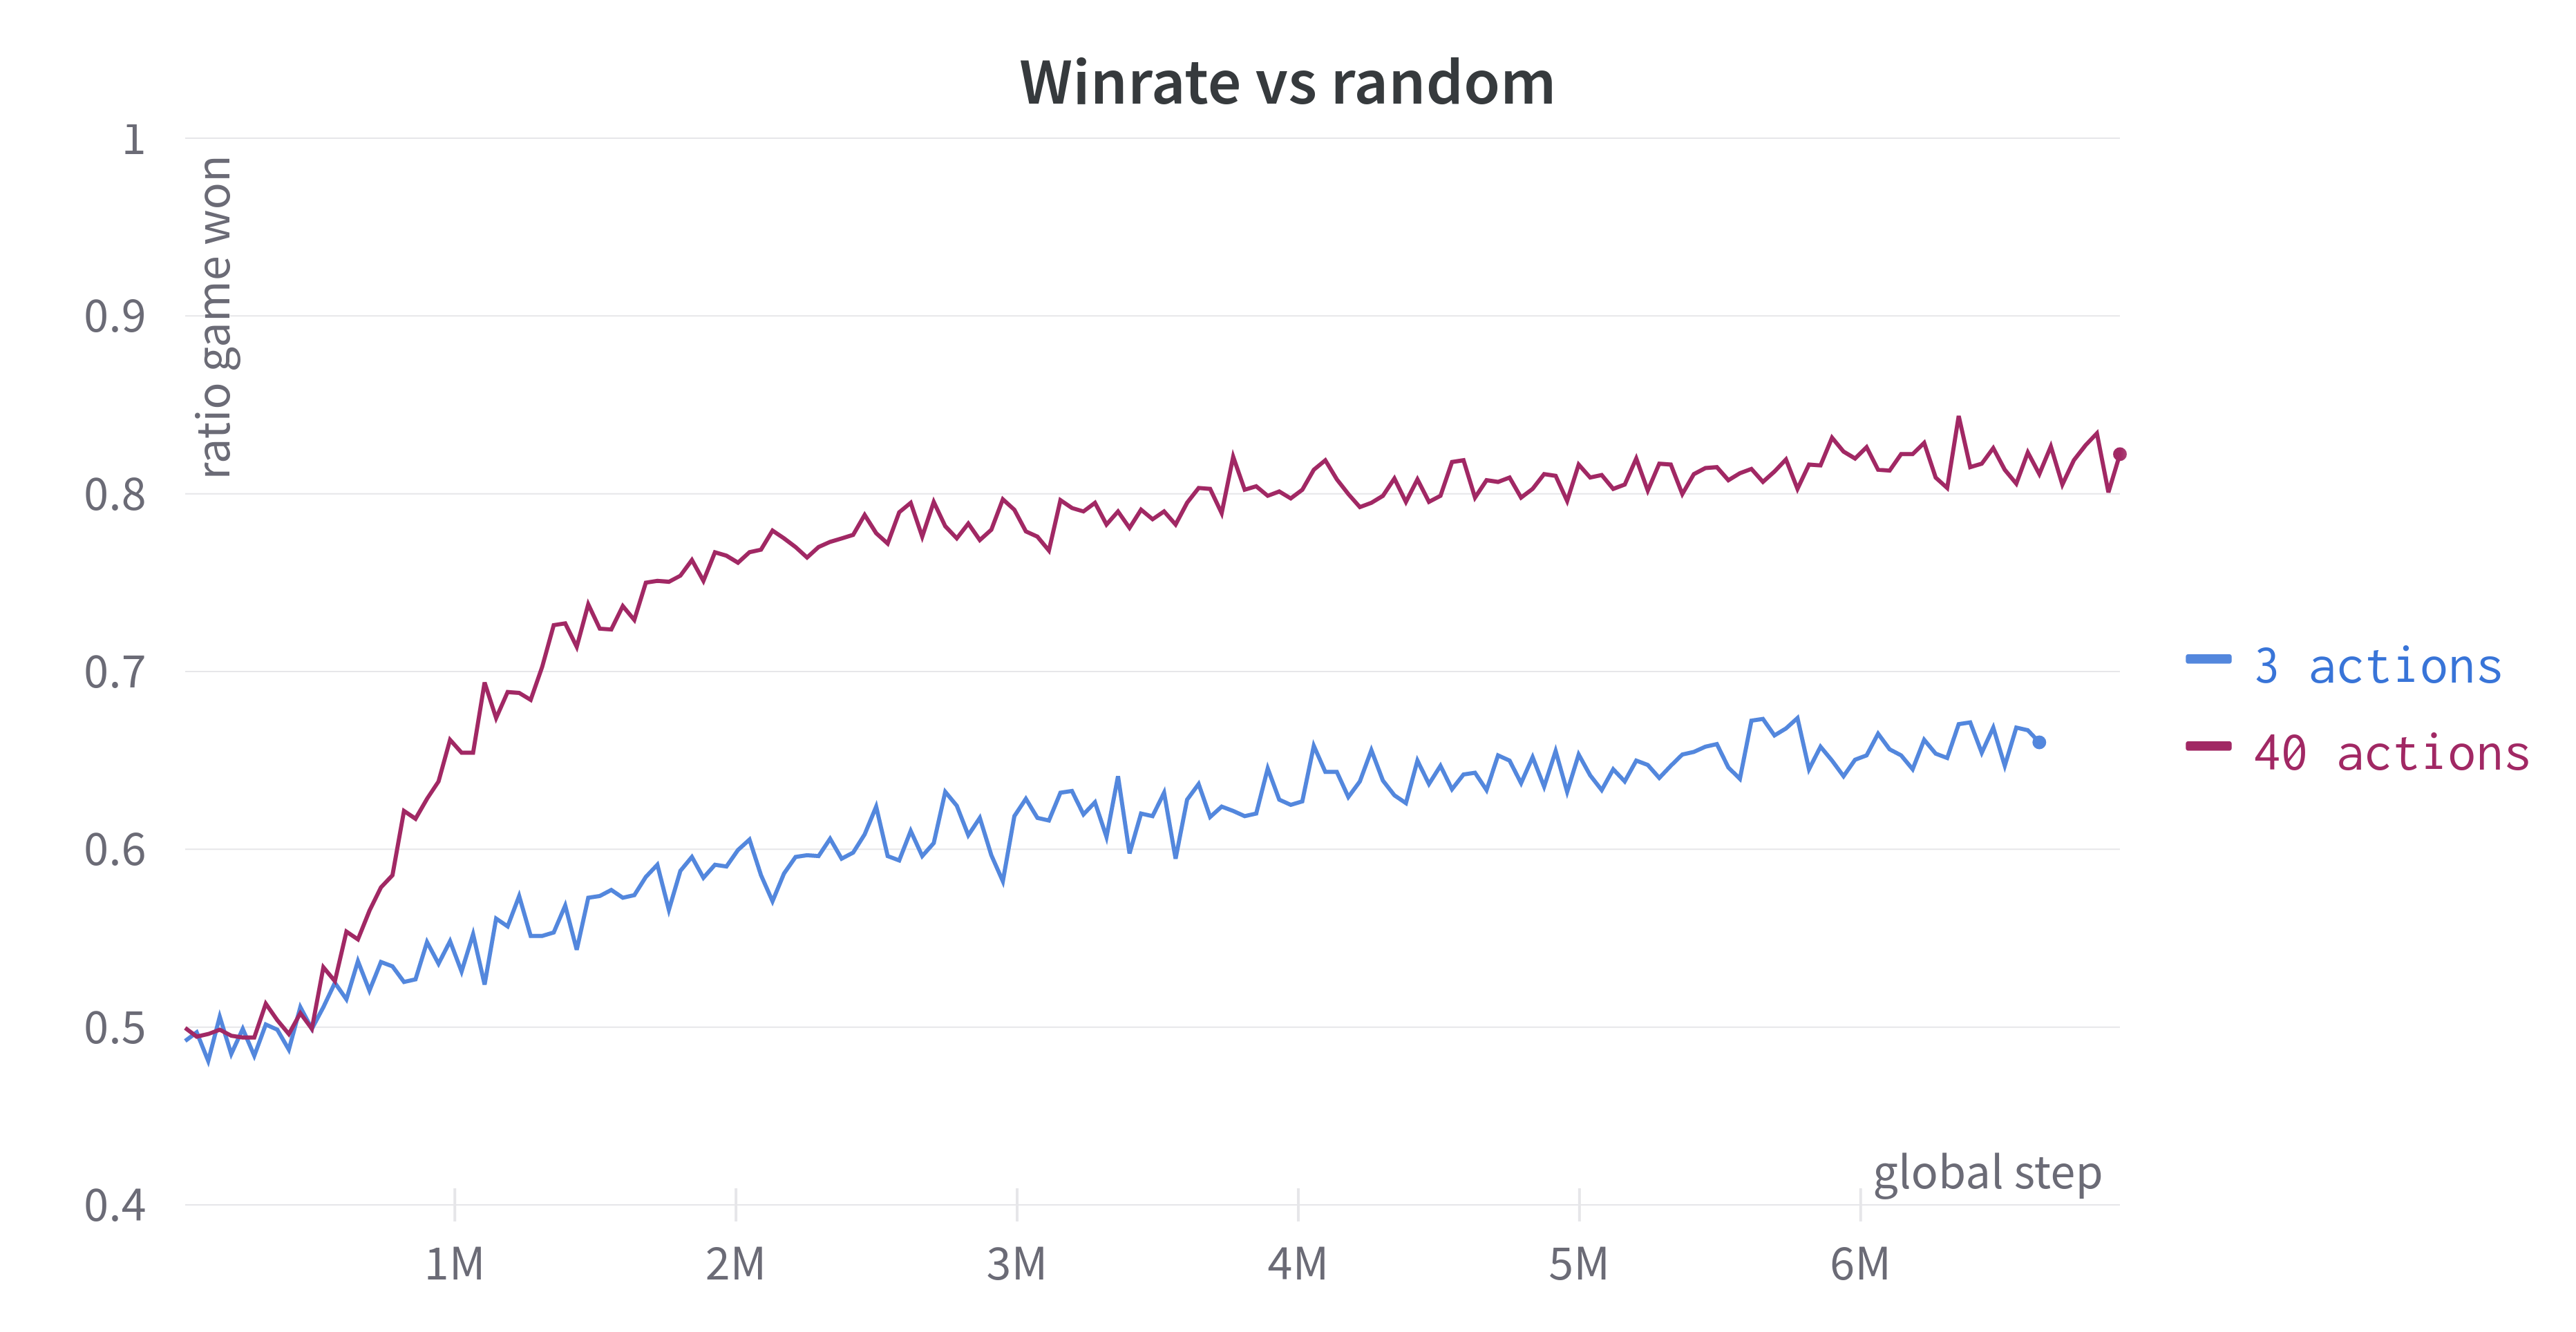
\includegraphics[width=\textwidth]{images/action-spaces-comparison.png}
    \caption{Performance of the two action space representations against a random player. The representation with 40 actions learns faster and reaches a win rate higher than 80\%, while the 3 action representation learns more slowly and reaches a win rate of 65\% by the end of training. In both representations we used invalid action masking as described in \cite{action-masking}.}
    \label{fig:action-space-comparison}
\end{figure}

\subsubsection{Invalid action masking}
Both in the first and second representation of the action space, the agent must not play a card that is not in its hand. This can be ensured through different methods, such as penalizing the agent for playing an invalid action or masking the invalid actions. We opted to implement the latter approach, as it has been shown empirically to be superior to penalizing invalid actions \cite{action-masking}.

The masking is done by setting the logits corresponding to the invalid actions to a small number, this way of performing the masking can be demonstrated to still produce a valid policy gradient as we are applying a differentiable state-dependent transformation to the policy \cite{action-masking}.

\begin{equation*}
    \pi'(\cdot|s) = \mathrm{softmax}(\mathrm{mask}(l(s)))
\end{equation*}
\begin{equation*}
    \mathrm{mask}(l_{i}) = \begin{cases}
        l_i & \text{if $a_i$ is valid} \\
        M & \text{otherwise}
    \end{cases}
\end{equation*}
Where $l$ is the logits vector, $a$ is the action vector, $s$ is the state and $M$ is a small number, in our implementation we used $M=-10^6$.

\subsection{Vectorized environment}
In order to make the training process faster, we utilized a vectorized environment. This is a wrapper around the original environment that allows multiple instances of it to run simultaneously. In this setup, the agent receives all observations from all environments at once, which enables batching of policy evaluation and potentially performing it on a GPU, resulting in a significant speed-up of the training process.

\section{Agent}


\section{Training procedure}